\documentclass[border=8pt,12pt]{standalone}
\usepackage{times}
\usepackage{inconsolata}
\usepackage[T1]{fontenc}
\usepackage{tikz}
\usetikzlibrary{arrows.meta, positioning, shadows}
\begin{document}
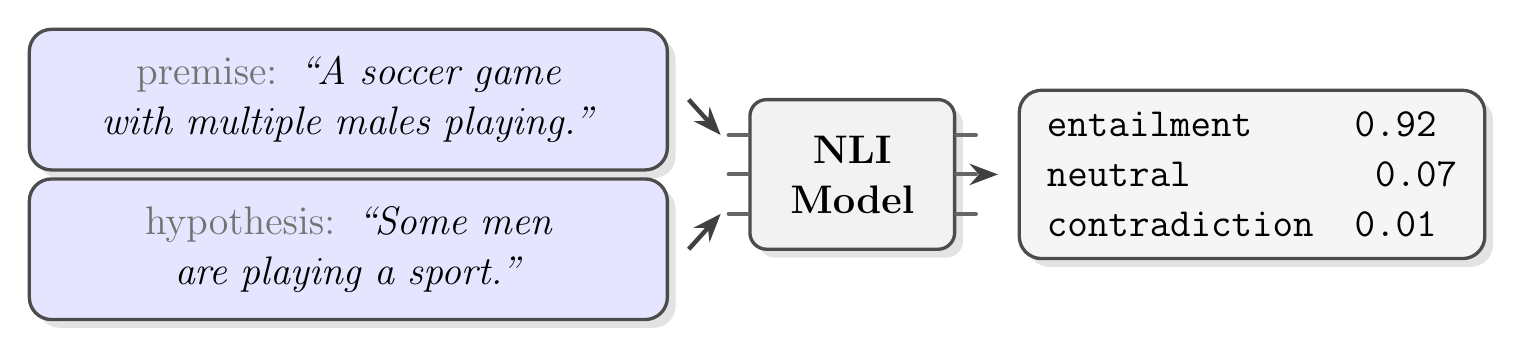
\begin{tikzpicture}[>=Stealth, font=\Large,
  card/.style={draw=black!70, line width=1.2pt, rounded corners=8pt, inner sep=10pt,
               drop shadow={opacity=0.22, shadow xshift=3pt, shadow yshift=-3pt}},
  nlcard/.style={card, fill=blue!10, text width=7.4cm, align=center, font=\Large\itshape},
  outcard/.style={card, fill=black!4, align=left, font=\Large\ttfamily, inner ysep=8pt},
  chip/.style={draw=black!70, line width=1.2pt, rounded corners=6pt, fill=black!5,
               minimum size=1.9cm, font=\Large\bfseries, inner sep=4pt,
               drop shadow={opacity=0.22, shadow xshift=3pt, shadow yshift=-3pt}},
  pin/.style={draw=black!60, line width=1.4pt, line cap=round},
  arr/.style={->, line width=1.6pt, black!75},
  lab/.style={font=\large, text=black!55},
]
\node[nlcard] (p) at (0, 0.95) {{\upshape\color{black!55}premise:} ``A soccer game with multiple males playing.''};
\node[nlcard] (h) at (0, -0.95) {{\upshape\color{black!55}hypothesis:} ``Some men are playing a sport.''};
\node[chip, minimum width=2.6cm, align=center] (nli) at (6.4, 0) {NLI\\Model};
\foreach \y in {-0.5,0,0.5} {
  \draw[pin] ([yshift=\y cm]nli.west) -- ++(-0.25,0);
  \draw[pin] ([yshift=\y cm]nli.east) -- ++(0.25,0);
}
\node[outcard, anchor=west] (o) at (8.5, 0) {entailment \ \ \ \ 0.92\\ neutral \ \ \ \ \ \ \ \ 0.07\\ contradiction \ 0.01};
\draw[arr] ([xshift=0.25cm]p.east) -- ([xshift=-0.35cm, yshift=0.5cm]nli.west);
\draw[arr] ([xshift=0.25cm]h.east) -- ([xshift=-0.35cm, yshift=-0.5cm]nli.west);
\draw[arr] ([xshift=0.35cm]nli.east) -- ([xshift=-0.25cm]o.west);
\end{tikzpicture}
\end{document}
